%************************************************
\chapter{Introduction}\label{ch:introduction}
%************************************************
\begin{flushleft}{\slshape    
    At the time, Nixon was normalizing relations with China.  
    I figured that if he could normalize relations, then so could I} \\ \medskip
    --- Edgar Codd
\end{flushleft}
%
Many modern data collections defy the traditional storage mechanisms of primary key based relational databases. With no natural ordering, it becomes either impossible or undesirable to index collections of this type.  For example, with a corpus of semi-structured data, or images on the world-wide-web, exact-match solutions, which have typified traditional databases, provide inadequate and often meaningless solutions.

As the number of such collections grow, there becomes a pressing need to address the problem of search.  In many cases, similarity searching provides the answer. Objects in a database can be thought of as points in a space that have a distance between them -- where similar objects are near each other.  The results of queries may be in terms of a region of the space, or as clusters within a region.  This thesis presents the results of questions pertaining to similarity searching.

In this introductory chapter, we present general metric spaces as an abstraction for working in similarity search; we examine techniques for partitioning space to assist with indexing; and thereafter, take a look at common search query types.
% ************************* %
 \section{Similarity search}
% ************************* %
Collections of unstructured or semi-structured data, where semantics are implicit in the data itself differ from relational databases, where the semantics of the data is contained in their schema.  Querying this type of data requires that \textit{features} representative of the semantics must first be extracted before any kind of comparison can be made.  Since it is often impossible to know \textit{a priori} what features will be present (as this will depend, to a large extent, on the domain), a natural question is how similar the respective feature sets are.  This is the essence of similarity search, which seeks to find other data which have similar semantics to a given data point.

Similarity search is increasingly playing a greater role in modern storage and retrieval techniques. In this paradigm, a distance between a query object and the objects stored in the database form the basis of the search. Objects that are close are highly similar, while objects that are far apart are dissimilar.  The result of a query then is the set of all objects that are close (or similar) to the query object.
More formally:
%
\begin{mydef} 
Given a collection $X$, and a query element $q$, retrieve all elements $x \in X$ that are \textit{similar}\footnote{We are deliberately vague about the definition of similar here, as there are numerous types of query available} to $q$. 
\end{mydef}
%
\noindent Applications for similarity search include: Optical character recognition;
 Statistical classification;
 Computer vision;
 Content-based image retrieval;
 Maximum likelihood decoding; 
 Data compression;
 Recommendation systems;
 Contextual advertising and behavioural targeting;
 DNA sequencing;
 Spelling checking; 
 Plagiarism detection; and 
 Cluster analysis.     
We now look more closely at some of these examples:
%
\ToDo{test To Do}
\begin{myexample}{Multimedia document retrieval}
One of the most common applications of SS is the retrieval of multimedia documents. E.g face recognition, object recognition, fingerprint matching, voice recognition, and multimedia databases in general. In this case the raw content of the document is not used, rather documents are processed for features.  Search is performed by comparing features.  Consider images, features extracted may be colours, textures, or shapes, represented as vectors.  One technique is to use each dimension of the vector to represent a colour and the size of each dimension is the number of pixels with that colour -- effectively a histogram.  The search then focuses on comparing the histograms.
\end{myexample}
%
\noindent 
%
\begin{myexample}{Recommender Systems}
By maintaining a profile of their users, recommender systems are able to suggest something new to a user (eg., to buy a book or visit a web-site).  In such cases the user's preferences are compared to other users' for similarity and suggestions are made on the basis that the user will like items that similar users do.
\end{myexample}
% 
% ********************** %
\section{Search queries}
% ********************** %
In general, there are two main types of query that are interesting: A range query, or a nearest-neighbour search.  A range query uses the distance function to effectively capture all elements that fall with in a particular radius of the query object.
  
\begin{mydef}
A range query is a function $R: S \times \mathbb{R} \rightarrow S$ such that $R(q, r) = \{y : d(q, x) < r\}$ where $r > 0$
\end{mydef}
%
\begin{myexample}{Range query example}
\end{myexample}
%
\begin{figure}
\centering
\subfloat[Range query] 
{\label{fig:range_query}
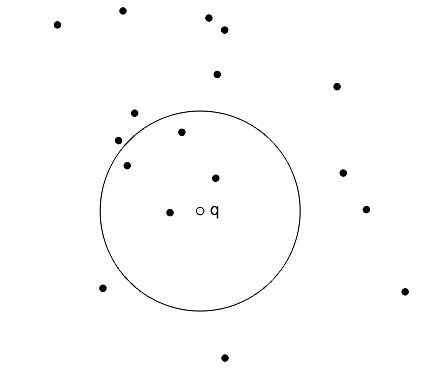
\includegraphics[width=.45\columnwidth]{gfx/range_query}} \quad
\subfloat[Nearest-Neighbour query] 
{\label{fig:nn_query}
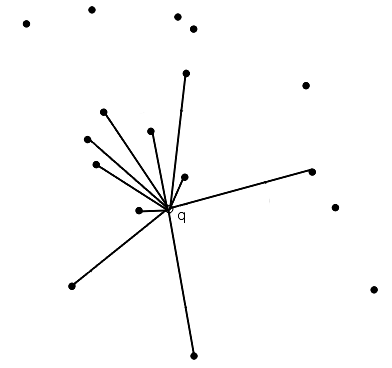
\includegraphics[width=.45\columnwidth]{gfx/nn_query}}
\caption[Range query and nearest-neighbours query in two dimensional Euclidean Space.]{Range query and nearest-neighbours query in two dimensional Euclidean Space.}
\end{figure}
%
\begin{mydef}
A nearest neighbour query is a function $NN:S \times \mathbb{Z}^+ \rightarrow S $ where $NN(q, k) = R \subseteq S$ such that $\forall x \in R, y \in S - R, d(q, x) < d(q,y) $ and $ |R| = k$.
\end{mydef}
%
\begin{myexample}{Nearest Neighbour query example}
\end{myexample}
